%%% app movel - funcionaliade
\begin{frame}{Aplicação Móvel - Funcionalidades}

\vspace*{-3em}

\begin{itemize}
	\item Funcionalidades
	\begin{itemize}
		\item consultar \textbf{voluntários, organizações, eventos e posts};
		\item permitir o registo e autenticação de voluntários através da aplicação;
		\item possibilitar aos utilizadores autenticados interagir com a plataforma (realização de \textit{posts}, seguimentos doutros utilizadores, etc.);
	\end{itemize}
\end{itemize}

\end{frame}

%%% app movel - arquiteture
\begin{frame}{Aplicação Móvel - Arquitetura}

\centering
\scalebox{0.30}{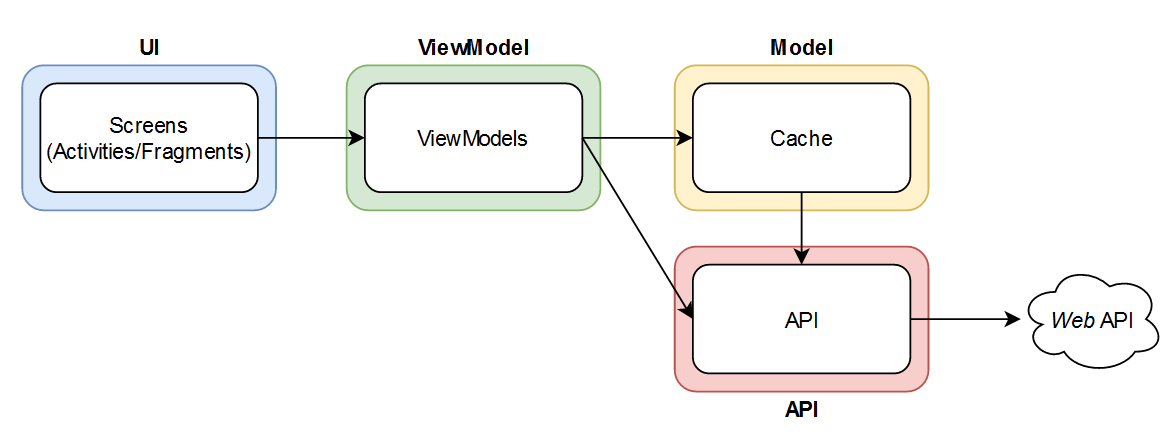
\includegraphics{Figures/mobile_app_architecture}}\\

\end{frame}